\documentclass[12pt]{article}

\usepackage{sbc-template}
\usepackage{graphicx,url}
\usepackage[utf8]{inputenc}
\usepackage[T1]{fontenc}
\usepackage[brazilian]{babel}

\sloppy

\title{LoraMind: Sistema de Comunicação Offline com Rede Mesh LoRa e Inteligência Artificial Local}

\author{Felipe Dias Konda\inst{1}, Ademar T. Akabane\inst{1}}

\address{
  Pontifícia Universidade Católica de Campinas\\
  Engenharia de Computação\\
  Campinas -- São Paulo -- Brasil
  \email{\{felipe.dk,ademar.akabane\}@puc-campinas.edu.br}
}

\begin{document}

\maketitle

% O resumo e o abstract serão escritos posteriormente.
% No artigo final em português, o modelo SBC normalmente exige os dois.

\section{Introdução}
\label{sec:introducao}

\subsection*{Contextualização do Problema}

Pessoas em regiões remotas ou envolvidas em situações de risco podem ficar sem acesso à Internet e à rede de telefonia celular justamente quando precisam de informações para decidir o que fazer. Esse cenário pode ocorrer, por exemplo, durante trilhas, viagens por áreas sem cobertura, falhas de veículos em locais afastados ou eventos que causem a interrupção da infraestrutura de comunicação. Sem conectividade, o usuário deixa de ter acesso a mecanismos de busca, aplicativos online e serviços de inteligência artificial que poderiam oferecer um direcionamento inicial.

Uma possível alternativa é disponibilizar um modelo de inteligência artificial diretamente no smartphone. Entretanto, os dispositivos Android apresentam grande variação de capacidade computacional. Enquanto aparelhos de alto desempenho possuem processadores mais rápidos e maior quantidade de memória, modelos de entrada operam com recursos significativamente mais limitados. A execução local de um modelo de linguagem também exige memória, capacidade de processamento e energia, podendo provocar lentidão, aquecimento, encerramento do aplicativo ou até impedir o funcionamento do sistema em parte dos dispositivos. Dessa forma, executar a inteligência artificial diretamente no celular reduziria a quantidade de usuários capazes de utilizar a solução.

\subsection*{Definição do Problema}

O problema central abordado neste trabalho é a dificuldade de fornecer orientações em linguagem natural a pessoas que se encontram sem acesso à Internet e que utilizam celulares sem capacidade suficiente para executar um modelo de inteligência artificial. A solução precisa, portanto, superar duas limitações: a ausência de um meio convencional de comunicação e a heterogeneidade de desempenho dos dispositivos Android.

Além disso, o celular deve permanecer apenas como uma interface acessível ao usuário, evitando que o funcionamento do sistema dependa de um aparelho de alto custo. O processamento mais pesado pode ser transferido para um equipamento com maior capacidade, desde que exista um meio de transportar as perguntas e respostas mesmo na ausência de Wi-Fi e dados móveis.

\subsection*{Apresentação da Solução}

Para atender a essas necessidades, foi desenvolvido o LoraMind, um sistema de comunicação offline que utiliza rádio LoRa para conectar o usuário a um modelo de linguagem executado em um computador. Essa divisão permite que o aplicativo Android seja responsável apenas pela interação com o usuário, enquanto o processamento da inteligência artificial ocorre em um equipamento mais potente e controlado.

No funcionamento proposto, o usuário digita uma pergunta no aplicativo Android e a mensagem é enviada por Bluetooth a um dispositivo ESP32 equipado com rádio LoRa. O pacote é transmitido pela rede mesh até uma estação-base conectada a um computador. Nesse computador, o modelo Gemma 2 é executado localmente por meio do Ollama, gera uma resposta e a devolve pelo caminho inverso. A resposta percorre a rede LoRa, chega novamente ao ESP32 do usuário e é apresentada no aplicativo.

Com essa arquitetura, não é necessário executar o modelo de linguagem no smartphone nem utilizar Internet, Wi-Fi ou dados móveis durante a comunicação. O uso de LoRa possibilita a transmissão de mensagens entre pontos afastados, enquanto os nós intermediários da rede mesh podem retransmitir os pacotes. Assim, celulares com diferentes níveis de desempenho podem acessar o mesmo modelo, pois a maior parte do processamento permanece concentrada na estação-base.

O LoraMind busca oferecer um direcionamento inicial em cenários nos quais outros meios de consulta estejam indisponíveis. As respostas geradas pela inteligência artificial, entretanto, não substituem profissionais, equipes de emergência ou serviços oficiais, devendo ser compreendidas como um recurso complementar em situações de conectividade limitada.

\subsection*{Objetivo do Trabalho}

O objetivo principal deste trabalho é desenvolver e analisar um sistema capaz de fornecer respostas geradas por inteligência artificial a usuários sem acesso à Internet, sem exigir que o modelo seja executado diretamente no dispositivo Android. Especificamente, o projeto busca:

\begin{itemize}
  \item disponibilizar uma interface Android para o envio de perguntas e a visualização das respostas;
  \item utilizar comunicação Bluetooth entre o smartphone e o nó LoRa;
  \item transmitir perguntas e respostas por uma rede mesh LoRa, sem depender de Wi-Fi ou dados móveis;
  \item executar o modelo de linguagem em um computador com maior capacidade de processamento;
  \item integrar os componentes de hardware e software em um fluxo de comunicação offline.
\end{itemize}

\section{Conceitos Fundamentais}
\label{sec:conceitos-fundamentais}

Esta seção apresenta os principais conceitos e tecnologias utilizados no desenvolvimento do LoraMind.

\subsection{Desenvolvimento Android}
\label{subsec:desenvolvimento-android}

O aplicativo do LoraMind foi desenvolvido em Kotlin para dispositivos Android. A seguir, são apresentados os principais conceitos utilizados em sua implementação.

\subsubsection{Jetpack Compose}

Jetpack Compose é o conjunto de ferramentas utilizado para construir a interface do aplicativo de forma declarativa. Nesse modelo, funções chamadas de \textit{composables} descrevem como a tela deve ser apresentada a partir dos dados atuais \cite{androidcomposestate2026}. No LoraMind, ele é empregado na tela de conversas, no campo de pergunta e na apresentação das respostas.

\subsubsection{Gerenciamento de Estado e Recomposição}

Estado é qualquer informação que pode variar durante o uso do aplicativo, como o texto digitado, a conversa selecionada e a espera por uma resposta. No LoraMind, a \textit{ViewModel} disponibiliza o estado da tela por meio de um \textit{StateFlow}, que é observado pelos componentes do Compose. Quando esse estado muda, o Compose executa a recomposição das partes afetadas da interface \cite{androidcomposestate2026}.

\subsubsection{MVVM}

O padrão MVVM (\textit{Model-View-ViewModel}) separa a interface, o estado da tela e os dados da aplicação. No LoraMind, os componentes do Compose formam a \textit{View}; a \textit{ChatViewModel} mantém o estado e trata as ações do usuário; e o \textit{Model} é representado pelas entidades, repositórios e regras da aplicação. Essa separação reduz a quantidade de lógica presente nas telas \cite{androidarchitecture2026}.

\subsubsection{Clean Architecture}

A Clean Architecture organiza o aplicativo em camadas com responsabilidades distintas. O projeto é dividido em apresentação, domínio e dados: a apresentação contém as telas e \textit{ViewModels}; o domínio reúne modelos, casos de uso e interfaces; e a camada de dados implementa a persistência e a comunicação Bluetooth. Essa organização limita a dependência direta entre a interface e os detalhes de implementação \cite{androidarchitecture2026}.

\subsubsection{Room}

Room é uma biblioteca de persistência que fornece uma camada de abstração sobre o SQLite \cite{androidroom2026}. No LoraMind, ela armazena localmente as conversas e mensagens por meio de entidades e objetos DAO (\textit{Data Access Object}). Os dados são disponibilizados como fluxos, permitindo atualizar a tela quando o histórico é alterado e mantê-lo disponível sem conexão com a Internet.

\subsubsection{Recepção de Mensagens por Socket Bluetooth}

O aplicativo estabelece uma conexão Bluetooth com o nó embarcado por meio de um \textit{BluetoothSocket}. O repositório monitora o fluxo de entrada do socket, lê os bytes disponíveis e emite a mensagem recebida em um \textit{Flow}; a \textit{ChatViewModel} coleta esse fluxo, salva a resposta e atualiza o estado da interface. Portanto, a recepção das respostas não utiliza um \textit{BroadcastReceiver}. Os protocolos empregados nessa conexão são apresentados na Subseção~\ref{subsubsec:spp-rfcomm}.

\subsection{Sistemas Embarcados}
\label{subsec:sistemas-embarcados}

Sistemas embarcados são dispositivos computacionais desenvolvidos para executar funções específicas e interagir diretamente com componentes eletrônicos. O LoraMind utiliza microcontroladores da família ESP32 para controlar os rádios LoRa e realizar a troca de mensagens entre o aplicativo, a rede e o computador.

\subsubsection{Dispositivos ESP32}

O nó conectado ao smartphone utiliza um ESP32, um módulo de comunicação LoRa e um display OLED SSD1306. O ESP32 executa o firmware, mantém a conexão Bluetooth e controla o rádio por meio do barramento SPI. A escolha desse modelo também permite utilizar Bluetooth Clássico na comunicação com o aplicativo \cite{espressifesp322026}.

A estação-base utiliza uma placa Heltec WiFi LoRa 32 V3.2, que integra um ESP32-S3, comunicação LoRa e uma interface USB serial \cite{espressifesp32s32026,heltecwifi32v32026}. O ESP32-S3 recebe os pacotes da rede e os encaminha ao programa executado no computador. Os dois dispositivos conseguem se comunicar quando são configurados com os mesmos parâmetros de rádio.

\subsubsection{Arduino IDE}

Arduino IDE é um ambiente utilizado para escrever, compilar e transferir programas, chamados de \textit{sketches}, para placas com microcontroladores. O ambiente também permite instalar pacotes de suporte para placas, adicionar bibliotecas e acompanhar mensagens pela porta serial \cite{arduinoide2026}. No LoraMind, ele é utilizado para gravar os arquivos \texttt{esp1.ino} no nó e \texttt{esp2.ino} na estação-base.

\subsubsection{LoRa}
\label{subsubsec:lora}

LoRa (\textit{Long Range}) é uma tecnologia de modulação de espectro espalhado destinada a enlaces sem fio de longo alcance e baixo consumo de energia \cite{semtechlora2026,augustin2016study}. Embora seja frequentemente chamado de protocolo, LoRa corresponde principalmente à camada física da comunicação. O LoraMind utiliza os rádios diretamente e define seu próprio protocolo sobre o enlace LoRa, sem empregar LoRaWAN.

Os rádios do projeto operam em 915~MHz, com largura de banda de 250~kHz, fator de espalhamento 7, taxa de codificação 4/5, potência de transmissão de 10~dBm, preâmbulo de oito símbolos e verificação CRC. Esses parâmetros precisam ser iguais nos dois dispositivos para que os pacotes sejam interpretados corretamente.

\subsubsection{Antenas}

A antena converte o sinal elétrico do rádio em ondas eletromagnéticas durante a transmissão e realiza o processo inverso na recepção. No protótipo, os dispositivos utilizam antenas compatíveis com a frequência de 915~MHz. A estação-base Heltec possui um conector IPEX para a antena LoRa externa \cite{heltecwifi32v32026}.

% TODO: confirmar o modelo, o tipo e o ganho das antenas utilizadas no protótipo.

\subsubsection{Biblioteca RadioLib}

RadioLib é uma biblioteca para o controle de diferentes módulos de comunicação sem fio \cite{radiolib2026}. No LoraMind, ela configura os parâmetros dos rádios, transmite os dados com a função \texttt{transmit()} e inicia a escuta com \texttt{startReceive()}. Quando o rádio recebe um pacote completo, um pino de interrupção altera uma variável de controle e o firmware realiza a leitura.

A RadioLib não define o cabeçalho utilizado pelo LoraMind. As funções \texttt{buildPacket()} e \texttt{parsePacket()}, implementadas no próprio firmware, são responsáveis por montar e interpretar a estrutura textual enviada pela biblioteca.

\subsubsection{Cabeçalho e Payload dos Pacotes}

Um pacote é formado por informações de controle e pelos dados transportados. O cabeçalho (\textit{header}) contém os campos necessários para identificar e encaminhar a mensagem, enquanto o \textit{payload} corresponde ao conteúdo útil destinado à aplicação. No LoraMind, foi definido o seguinte formato:

\begin{center}
  \texttt{LM|TIPO|MSG\_ID|TTL|payload}
\end{center}

O prefixo \texttt{LM} identifica mensagens pertencentes ao sistema; \texttt{TIPO} informa se o pacote contém uma pergunta (\texttt{Q}) ou resposta (\texttt{R}); \texttt{MSG\_ID} identifica a mensagem; e \texttt{TTL} limita a quantidade de retransmissões. Esses campos formam o cabeçalho de aplicação criado para o LoraMind. O campo \texttt{payload} transporta a pergunta ou a resposta. Esse cabeçalho não deve ser confundido com as informações acrescentadas pelo próprio rádio durante a transmissão.

\subsubsection{Relay e Rede Mesh}
\label{subsubsec:relay-mesh}

Relay é a retransmissão de um pacote por um nó intermediário. Quando um dispositivo recebe uma mensagem que não deve ser entregue localmente, ele reduz o campo \texttt{TTL} e transmite o pacote novamente. Se o valor chegar a zero, o pacote é descartado. Cada nó também mantém um registro temporário dos identificadores recebidos para evitar que uma mesma mensagem seja retransmitida repetidamente.

Uma rede mesh permite que os dispositivos cooperem no encaminhamento das mensagens, formando uma comunicação de múltiplos saltos \cite{poke2023empirical}. Dessa forma, um nó que não alcança diretamente a estação-base pode utilizar outros nós como relays. A implementação do LoraMind não mantém uma tabela de rotas: perguntas novas são retransmitidas em direção à rede, e as respostas são entregues ao nó que possui o identificador como pendente ou retransmitidas pelos demais nós. O TTL e a deduplicação limitam essa propagação.

\subsubsection{SPP e RFCOMM}
\label{subsubsec:spp-rfcomm}

SPP (\textit{Serial Port Profile}) é um perfil do Bluetooth Clássico que permite simular uma conexão serial entre dois dispositivos. Essa comunicação utiliza o RFCOMM, protocolo orientado a conexão que fornece um fluxo contínuo de bytes sobre o enlace Bluetooth \cite{bluetoothsigsp,androidbluetooth2026}. No LoraMind, o ESP32 disponibiliza o serviço SPP por meio da classe \texttt{BluetoothSerial}, enquanto o aplicativo Android se conecta a ele utilizando um \textit{BluetoothSocket} RFCOMM. Após a conexão, os fluxos de entrada e saída transportam perguntas e respostas entre o aplicativo e o nó embarcado.

\subsection{Inteligência Artificial Local}
\label{subsec:inteligencia-artificial-local}

Na execução local, o modelo de inteligência artificial permanece no próprio computador e pode funcionar sem acessar serviços de nuvem. Essa abordagem permite concentrar o processamento em um equipamento com maior capacidade, evitando que o modelo precise ser executado em cada smartphone.

\subsubsection{Ollama}

O Ollama é uma ferramenta que permite baixar, gerenciar e executar modelos de linguagem no próprio computador. Durante sua execução, ele mantém um serviço local responsável por carregar o modelo escolhido e disponibiliza uma API HTTP para que outros programas enviem perguntas e recebam as respostas geradas \cite{ollamaapi2026}. Depois que o Ollama e o modelo estão instalados, essa comunicação ocorre no próprio computador, sem que as perguntas precisem ser encaminhadas a um serviço de inteligência artificial na nuvem.

\subsubsection{Modelo Gemma 2}

Gemma é uma família de modelos de linguagem desenvolvida pelo Google. Esses modelos recebem texto como entrada e produzem texto como saída, podendo ser empregados em tarefas como perguntas e respostas, resumo e geração de conteúdo. O LoraMind utiliza a variante Gemma 2 9B, identificada no Ollama como \texttt{gemma2:9b}, por oferecer uma relação adequada entre capacidade de geração e viabilidade de execução em um computador pessoal \cite{gemmateam2024gemma2}.

O programa fornece ao modelo um conjunto de instruções que define o comportamento esperado do assistente, incluindo respostas curtas e orientações voltadas a situações em que o usuário não possui acesso à Internet ou à rede de telefonia. Também são mantidas até cinco interações anteriores de cada conversa, permitindo que o modelo considere mensagens já trocadas ao produzir uma nova resposta.

\subsubsection{Ponte Python e Porta Serial}

A integração entre a estação-base e a inteligência artificial é realizada pelo programa \texttt{loramind\_bridge.py}. O programa identifica as portas seriais disponíveis no computador e procura a interface USB associada ao ESP32. Em seguida, abre a porta COM selecionada a 115200 baud por meio da biblioteca \textit{pySerial}, que fornece operações de leitura e escrita em interfaces seriais \cite{pyserial2026}.

Essa comunicação não utiliza um socket. No Windows, a conexão USB serial do ESP32 é representada por uma porta COM. O programa permanece em um laço de leitura utilizando \texttt{readline()}, aguardando linhas enviadas pela estação-base. Apenas mensagens no formato \texttt{MSG\_LORAMIND:MSG\_ID|payload} são interpretadas e encaminhadas ao modelo; as demais linhas recebidas são ignoradas.

\subsubsection{Chamada à API do Ollama}

Após extrair a pergunta recebida pela porta serial, o programa monta uma requisição em formato JSON com o nome do modelo, as instruções do sistema, o histórico da conversa e a mensagem do usuário. A requisição é enviada com o método HTTP \texttt{POST} para o endereço local \texttt{http://localhost:11434/api/chat}, utilizando a biblioteca \textit{Requests} \cite{ollamaapi2026}.

A API devolve a resposta gradualmente, por meio de transmissão contínua. O programa reúne os trechos recebidos, limita o histórico da conversa e divide textos longos em partes compatíveis com os pacotes usados pelo sistema. Por fim, cada parte é escrita na porta serial no formato \texttt{RESP\_AI:MSG\_ID|resposta}, para que o ESP32 da estação-base a transmita pela rede LoRa.

Como conteúdos gerados por inteligência artificial podem apresentar informações incorretas, as respostas do sistema devem ser consideradas direcionamentos complementares e não substituem profissionais ou serviços oficiais de emergência.

\section{Arquitetura de Software}

\subsection{Arquitetura Geral}
\label{subsec:arquitetura-geral}

A arquitetura geral do LoraMind integra o aplicativo Android, o nó ESP32 conectado ao usuário, a rede LoRa, o ESP32 da estação-base e o computador responsável pela execução local do modelo de inteligência artificial. A Figura~\ref{fig:arquitetura-geral} apresenta os principais componentes e os canais de comunicação utilizados entre eles.

\begin{center}
  \centering
  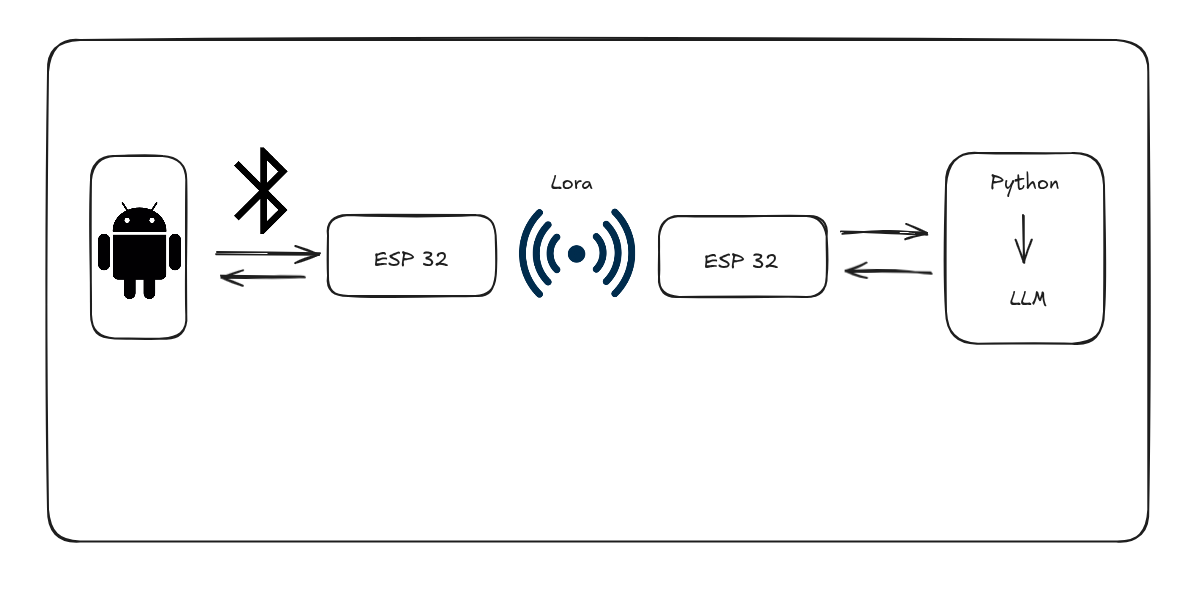
\includegraphics[width=\textwidth]{figuras/loramind-arquitetura.png}
  \captionof{figure}{Arquitetura geral do LoraMind.}
  \label{fig:arquitetura-geral}
\end{center}

O fluxo de envio começa quando o usuário conecta o aplicativo ao nó ESP32 por Bluetooth e escreve uma pergunta. O aplicativo envia o texto pelo fluxo de saída do \textit{BluetoothSocket} RFCOMM. Ao receber a linha pelo serviço SPP, o firmware do nó gera um identificador para a mensagem e monta um pacote de pergunta no formato \texttt{LM|Q|MSG\_ID|TTL|payload}. Esse pacote é então transmitido pelo rádio LoRa e pode ser retransmitido pelos nós intermediários até alcançar a estação-base.

Quando o ESP32 da estação-base recebe o pacote LoRa, o firmware realiza o \textit{parsing} da mensagem. O prefixo \texttt{LM} permite verificar se o pacote pertence ao protocolo do LoraMind; em seguida, são extraídos o tipo, o identificador, o TTL e o \textit{payload}. Se o pacote for válido e representar uma pergunta, a estação-base encaminha seu conteúdo ao computador pela conexão USB serial no formato \texttt{MSG\_LORAMIND:MSG\_ID|payload}.

No computador, o programa Python lê a pergunta da porta COM e a envia à API local do Ollama. O modelo Gemma 2 gera a resposta, que é recebida pelo programa e escrita de volta na porta serial no formato \texttt{RESP\_AI:MSG\_ID|resposta}. A estação-base identifica esse prefixo, recupera o identificador e o conteúdo, monta um pacote LoRa do tipo resposta, \texttt{LM|R|MSG\_ID|TTL|payload}, e o transmite pela rede.

Ao receber um pacote de resposta, o nó ESP32 verifica se o identificador corresponde a uma pergunta enviada por ele. Em caso positivo, o \textit{payload} é encaminhado ao smartphone por Bluetooth. No aplicativo, o repositório monitora o fluxo de entrada do \textit{BluetoothSocket} e emite o texto recebido para a \textit{ChatViewModel}. A \textit{ViewModel} cria uma mensagem identificada como resposta da inteligência artificial, salva-a no banco de dados local e atualiza o estado da interface, fazendo com que o conteúdo seja apresentado na tela ao usuário.

\subsection{Arquitetura do Aplicativo Android}
\label{subsec:arquitetura-aplicativo}

O aplicativo Android foi organizado com base na Clean Architecture e no padrão MVVM. A Clean Architecture divide o código nas camadas de apresentação, domínio e dados, enquanto o MVVM separa a interface construída com Jetpack Compose do estado e das ações controladas pela \textit{ChatViewModel} \cite{androidarchitecture2026}. Essa organização foi escolhida para manter as responsabilidades bem definidas e reduzir o acoplamento entre a interface, as regras da aplicação, a comunicação Bluetooth e o banco de dados.

A camada de apresentação exibe os dados e encaminha as ações do usuário; a camada de domínio reúne os modelos e as regras da aplicação; e a camada de dados implementa o acesso ao Bluetooth e à persistência local. Dessa forma, uma alteração no mecanismo de armazenamento ou comunicação pode ser realizada com menor impacto sobre as telas, facilitando a manutenção, os testes e a evolução do código.

\subsubsection{Camada de Dados}

A camada de dados contém as implementações dos repositórios e os mecanismos utilizados para acessar fontes externas. Para a persistência local, o LoraMind utiliza a biblioteca Room, que fornece uma abstração sobre o SQLite \cite{androidroom2026}. As classes \texttt{MessageEntity} e \texttt{ConversationEntity} representam as tabelas de mensagens e conversas, enquanto os DAOs \texttt{MessageDao} e \texttt{ConversationDao} definem as operações de consulta, inserção, atualização e remoção. A classe \texttt{AppDatabase} configura o banco e disponibiliza esses DAOs.

A implementação do repositório de mensagens utiliza o \texttt{MessageDao}, enquanto o repositório de conversas utiliza o \texttt{ConversationDao}. Ambos convertem as entidades armazenadas para os modelos empregados pelas demais camadas. A comunicação com o dispositivo embarcado é implementada por \texttt{BluetoothRepositoryImpl}, que utiliza a API nativa de Bluetooth do Android para localizar o dispositivo, criar um \textit{BluetoothSocket} RFCOMM com o serviço SPP e acessar seus fluxos de entrada e saída \cite{androidbluetooth2026}. As mensagens recebidas são disponibilizadas por meio de um \textit{Flow}, sem expor os detalhes do socket às outras camadas.

\subsubsection{Camada de Domínio}

A camada de domínio concentra as definições que representam as regras centrais do aplicativo e não depende diretamente das classes do Room ou da API Bluetooth do Android. O modelo \texttt{Conversation} possui os campos \texttt{id}, identificador único da conversa; \texttt{title}, título apresentado ao usuário; \texttt{createdAt}, instante de criação; e \texttt{updatedAt}, instante da última atualização. Esses dois últimos campos permitem registrar a data da conversa e ordenar as conversas pela modificação mais recente.

O modelo \texttt{Message} possui os campos \texttt{id}, identificador único da mensagem; \texttt{text}, conteúdo enviado ou recebido; \texttt{isFromUser}, que indica se a mensagem foi escrita pelo usuário ou gerada pela inteligência artificial; \texttt{timestamp}, instante em que a mensagem foi criada; e \texttt{conversationId}, identificador da conversa à qual ela pertence.

A relação entre os dados é de uma conversa para várias mensagens. Ao criar uma mensagem, a \textit{ChatViewModel} copia o \texttt{id} da conversa ativa para o campo \texttt{conversationId}. Para carregar o histórico, o \texttt{MessageDao} seleciona somente os registros cujo \texttt{conversationId} seja igual ao identificador da conversa selecionada e os ordena pelo \texttt{timestamp}. Assim, mesmo que existam mensagens de várias conversas na mesma tabela, o aplicativo apresenta apenas as associadas à conversa ativa. No banco atual, essa associação é controlada pela aplicação, pois \texttt{conversationId} funciona como campo de vínculo, mas não foi declarado como uma chave estrangeira do Room. Ao excluir uma conversa, a \textit{ViewModel} remove primeiro suas mensagens utilizando esse identificador e, em seguida, remove a própria conversa.

A interface \texttt{MessageRepository} define as operações relacionadas às mensagens, e \texttt{ConversationRepository} define as operações das conversas. Por sua vez, \texttt{BluetoothRepository} estabelece as operações de conexão, envio e recebimento pelo Bluetooth. As implementações concretas dessas interfaces permanecem na camada de dados.

Os casos de uso representam ações específicas da aplicação. No LoraMind, o \texttt{SendMessageUseCase} verifica se a mensagem não está vazia e solicita seu envio por meio da interface \texttt{BluetoothRepository}. Como o domínio depende da interface, e não de \texttt{BluetoothRepositoryImpl}, o mecanismo de comunicação pode ser substituído por outra implementação, como o repositório simulado existente no projeto, sem alterar a regra do caso de uso.

\subsubsection{Camada de Apresentação}

A camada de apresentação reúne a tela construída com Jetpack Compose, a \textit{ViewModel} e o estado da interface. A função \texttt{ChatScreen} representa a tela principal do aplicativo. Ela observa o estado fornecido pela \texttt{ChatViewModel}, apresenta as conversas e mensagens e encaminha ações como digitar, enviar, selecionar ou excluir uma conversa. Dessa forma, a tela fica responsável pela exibição e delega o tratamento das ações à \textit{ViewModel}.

Entre os componentes do Compose utilizados, a \texttt{LazyColumn} apresenta a lista de mensagens e cria um \texttt{ChatBubble} para cada item da conversa ativa. Esse componente é apropriado para listas que podem crescer, pois organiza os elementos verticalmente e compõe os itens conforme eles são necessários. O \texttt{TextField}, presente em \texttt{ChatInputBar}, exibe o texto de entrada armazenado no estado; a cada alteração, chama a \textit{ViewModel} para atualizar esse valor. O botão de envio chama \texttt{sendMessage()} e permanece desabilitado quando o campo está vazio ou quando o aplicativo aguarda uma resposta.

A \texttt{ChatViewModel} funciona como intermediária entre a tela e as camadas de domínio e dados. Ela executa o caso de uso de envio, observa as conversas e mensagens armazenadas, recebe as respostas do Bluetooth e atualiza um \texttt{StateFlow} do tipo \texttt{ChatUiState}. Esse estado reúne a lista de mensagens, o texto digitado, a indicação de espera pela resposta, a lista de conversas, a conversa ativa e o estado do menu lateral. A \texttt{ChatScreen} converte o fluxo em um estado do Compose com \texttt{collectAsState()}; quando um desses valores muda, as partes dependentes da interface são recompostas \cite{androidcomposestate2026}.

A \texttt{MainActivity} é o ponto de entrada do aplicativo. Em \texttt{onCreate()}, o método \texttt{setContent()} inicia a árvore de componentes do Compose, aplica o tema do LoraMind e apresenta a \texttt{ChatScreen} \cite{androidcomposeviews2026}. A atividade também solicita as permissões necessárias de acordo com a versão do Android e realiza a composição das dependências: obtém o banco e os DAOs, cria os repositórios e o caso de uso, instancia a \texttt{ChatViewModel} por meio de uma fábrica e a fornece à tela.

\subsection{Arquitetura dos Dispositivos ESP32}
\label{subsec:arquitetura-esp32}

\subsubsection{Nó Conectado ao Smartphone}

O nó próximo ao usuário é formado por um ESP32 com Bluetooth Clássico, rádio LoRa, antena de 915~MHz e display OLED. O firmware mantém um serviço SPP para receber as perguntas do aplicativo e enviar as respostas. O display apresenta informações básicas de funcionamento, enquanto o rádio permite que o nó participe da rede sem depender de Wi-Fi ou dados móveis.

A comunicação LoRa é controlada pela biblioteca RadioLib \cite{radiolib2026}. Durante a inicialização, o firmware configura os parâmetros do rádio e registra a função de interrupção usada para indicar a chegada de dados. A transmissão é realizada com \texttt{transmit()}, a escuta é iniciada por \texttt{startReceive()} e o conteúdo recebido é obtido com \texttt{readData()}. A RadioLib transporta a sequência de caracteres; a montagem e a interpretação do protocolo do LoraMind permanecem sob responsabilidade do firmware.

\subsubsection{Estrutura do Pacote}

Antes de transmitir uma mensagem, a função \texttt{buildPacket()} organiza os dados no formato \texttt{LM|TIPO|MSG\_ID|TTL|payload}. Os quatro primeiros campos formam o cabeçalho de aplicação. \texttt{LM} é o prefixo fixo usado para reconhecer mensagens do LoraMind; \texttt{TIPO} recebe \texttt{Q} para pergunta ou \texttt{R} para resposta; \texttt{MSG\_ID} é um identificador alfanumérico de quatro caracteres; e \texttt{TTL} informa quantas retransmissões ainda podem ocorrer. O \texttt{payload} contém o texto da pergunta ou da resposta e pode incluir o identificador da conversa antes do texto.

Na recepção, \texttt{parsePacket()} separa os campos pelos caracteres \texttt{|} e verifica o prefixo, o tipo, o identificador e o TTL. Pacotes com estrutura inválida ou sem o prefixo \texttt{LM} são descartados. Quando a validação é concluída, o firmware utiliza o tipo e o identificador para decidir se deve entregar, retransmitir ou ignorar a mensagem.

\subsubsection{Encaminhamento na Rede Mesh}

O protocolo não inclui um endereço de origem ou destino para cada nó. Uma pergunta do tipo \texttt{Q} é sempre destinada à estação-base. Por isso, quando um nó comum recebe uma pergunta que ainda não está em seu registro de mensagens vistas, ele reduz o TTL e a retransmite; perguntas duplicadas ou com TTL igual a zero são descartadas. A estação-base é o único dispositivo que consome a pergunta e a encaminha ao computador.

Quando o nó envia uma pergunta criada pelo aplicativo, ele guarda o respectivo \texttt{MSG\_ID} em uma lista de mensagens pendentes. Ao receber uma resposta do tipo \texttt{R}, verifica se o identificador está nessa lista. Se estiver, a resposta pertence àquele nó e seu \texttt{payload} é enviado ao smartphone por Bluetooth. Caso contrário, o TTL é reduzido e a resposta é retransmitida. O registro de mensagens já recebidas evita ciclos e transmissões repetidas; para respostas divididas em partes, a deduplicação considera o identificador junto com o conteúdo de cada parte.

\subsubsection{Estação-base Conectada ao Computador}

A estação-base utiliza uma placa Heltec com ESP32-S3, comunicação LoRa, antena de 915~MHz e interface USB serial. Quando recebe uma pergunta válida e ainda não processada, o firmware remove o cabeçalho da rede e escreve na serial a linha \texttt{MSG\_LORAMIND:MSG\_ID|payload}. O programa Python lê essa linha, envia a pergunta ao modelo e devolve a resposta como \texttt{RESP\_AI:MSG\_ID|resposta}.

O firmware da estação-base lê a resposta da serial, recupera o \texttt{MSG\_ID} e o texto e monta um novo pacote do tipo \texttt{R}. Depois da transmissão, volta ao modo de escuta. Como uma resposta pode retornar à estação-base após ser retransmitida por outros nós, o firmware mantém um registro das respostas enviadas e ignora esses ecos, evitando que sejam processados novamente.

\subsection{Modelo Local de Inteligência Artificial}
\label{subsec:modelo-local-ia}

\subsubsection{Ponte em Python}

O arquivo \texttt{loramind\_bridge.py} realiza a integração entre o ESP32 da estação-base e o modelo de inteligência artificial. Ao ser iniciado, o programa procura uma porta serial associada ao ESP32, priorizando interfaces USB conhecidas, ou utiliza a porta COM informada pelo usuário. A comunicação é aberta a 115200 baud com a biblioteca \textit{pySerial} \cite{pyserial2026}.

O programa permanece lendo as linhas recebidas e processa somente aquelas iniciadas por \texttt{MSG\_LORAMIND:}. Em seguida, separa o \texttt{MSG\_ID}, o identificador da conversa e a pergunta. O identificador da conversa permite manter separadamente até cinco trocas anteriores de cada usuário, que são acrescentadas à nova requisição para preservar o contexto.

O script também prepara a entrada e a saída para as limitações do sistema. Um \textit{prompt} de sistema orienta o modelo a produzir respostas diretas, em texto simples e com duas ou três frases, além de priorizar ações que possam ser realizadas sem Internet ou telefonia em situações de risco. Depois da geração, o texto é limpo e, caso ultrapasse 200 caracteres, dividido sem cortar palavras. Cada parte é então enviada ao ESP32 no formato \texttt{RESP\_AI:MSG\_ID|resposta}, com um intervalo de dois segundos entre partes consecutivas.

\subsubsection{Ollama e API Local}

O Ollama é responsável por armazenar, carregar e executar o modelo no computador, disponibilizando seu acesso por meio de uma API HTTP local \cite{ollamaapi2026}. Antes de iniciar o fluxo principal, o script consulta \texttt{/api/tags} para verificar se o serviço está ativo e se o modelo configurado está disponível.

Para gerar uma resposta, o programa envia uma requisição HTTP \texttt{POST} para \texttt{http://localhost:11434/api/chat}. O corpo JSON contém o nome do modelo, o \textit{prompt} de sistema, o histórico da conversa, a pergunta atual e os parâmetros de geração. A opção de transmissão contínua permanece habilitada, fazendo com que a API devolva os trechos conforme são produzidos. O script reúne esses trechos até receber a indicação de término e somente então prepara a resposta para a porta serial.

\subsubsection{Modelo e Parâmetros Utilizados}

O modelo selecionado para a versão atual é o Gemma 2 9B, identificado no Ollama como \texttt{gemma2:9b}. Ele possui aproximadamente 9,2 bilhões de parâmetros e janela de contexto de até 8.192 tokens \cite{gemmateam2024gemma2}. No LoraMind, a temperatura foi configurada em 0,6 e o limite de geração em 150 tokens. Esses valores, combinados ao histórico reduzido e ao \textit{prompt} de sistema, buscam equilibrar consistência, concisão e tempo de processamento.

Durante o desenvolvimento também foi testado o modelo \texttt{qwen2.5:3b}. Embora seja menor, nos testes realizados ele apresentou menor aderência às instruções específicas do projeto, chegando a recomendar recursos externos, como realizar ligações, mesmo em cenários definidos como sem cobertura de telefonia. O Gemma 2 9B apresentou respostas mais adequadas ao contexto e melhor cumprimento do formato solicitado, motivo pelo qual foi adotado na versão atual. Essa escolha corresponde aos testes funcionais do protótipo e não a uma avaliação comparativa formal entre os modelos.

Nos testes do sistema, a geração pelo modelo ocorreu normalmente em aproximadamente três a cinco segundos. Considerando também o envio da pergunta, o processamento da estação-base, a divisão da resposta e seu retorno pela rede, o tempo total observado ficou geralmente entre cinco e dez segundos. Esses valores podem variar conforme o computador utilizado, o tamanho da pergunta e da resposta e a quantidade de retransmissões na rede LoRa.

\section{Interfaces do Sistema}
\label{sec:interfaces-sistema}

O LoraMind possui duas formas de acompanhamento: a interface do aplicativo Android, utilizada pelo usuário para enviar perguntas e receber respostas, e a interface textual apresentada no terminal do computador, utilizada para acompanhar a comunicação com a estação-base e o modelo local de inteligência artificial.

\subsection{Interface do Aplicativo Android}

\subsubsection{Acesso e Estado Inicial}

O aplicativo é identificado no menu do Android pelo nome LoraMind e por um ícone próprio, conforme a Figura~\ref{fig:acesso-estado-inicial}(a). Após a abertura, a tela inicial apresenta o nome do sistema, o acesso ao histórico, indicadores de comunicação e a identificação \textit{Offline AI}. Quando a conversa ainda não possui mensagens, a região central apresenta uma orientação para que o usuário inicie a interação, como mostra a Figura~\ref{fig:acesso-estado-inicial}(b). O campo de texto e o botão de envio permanecem disponíveis na parte inferior.

\begin{figure}[htbp]
    \centering
    \begin{minipage}[t]{0.46\textwidth}
        \centering
        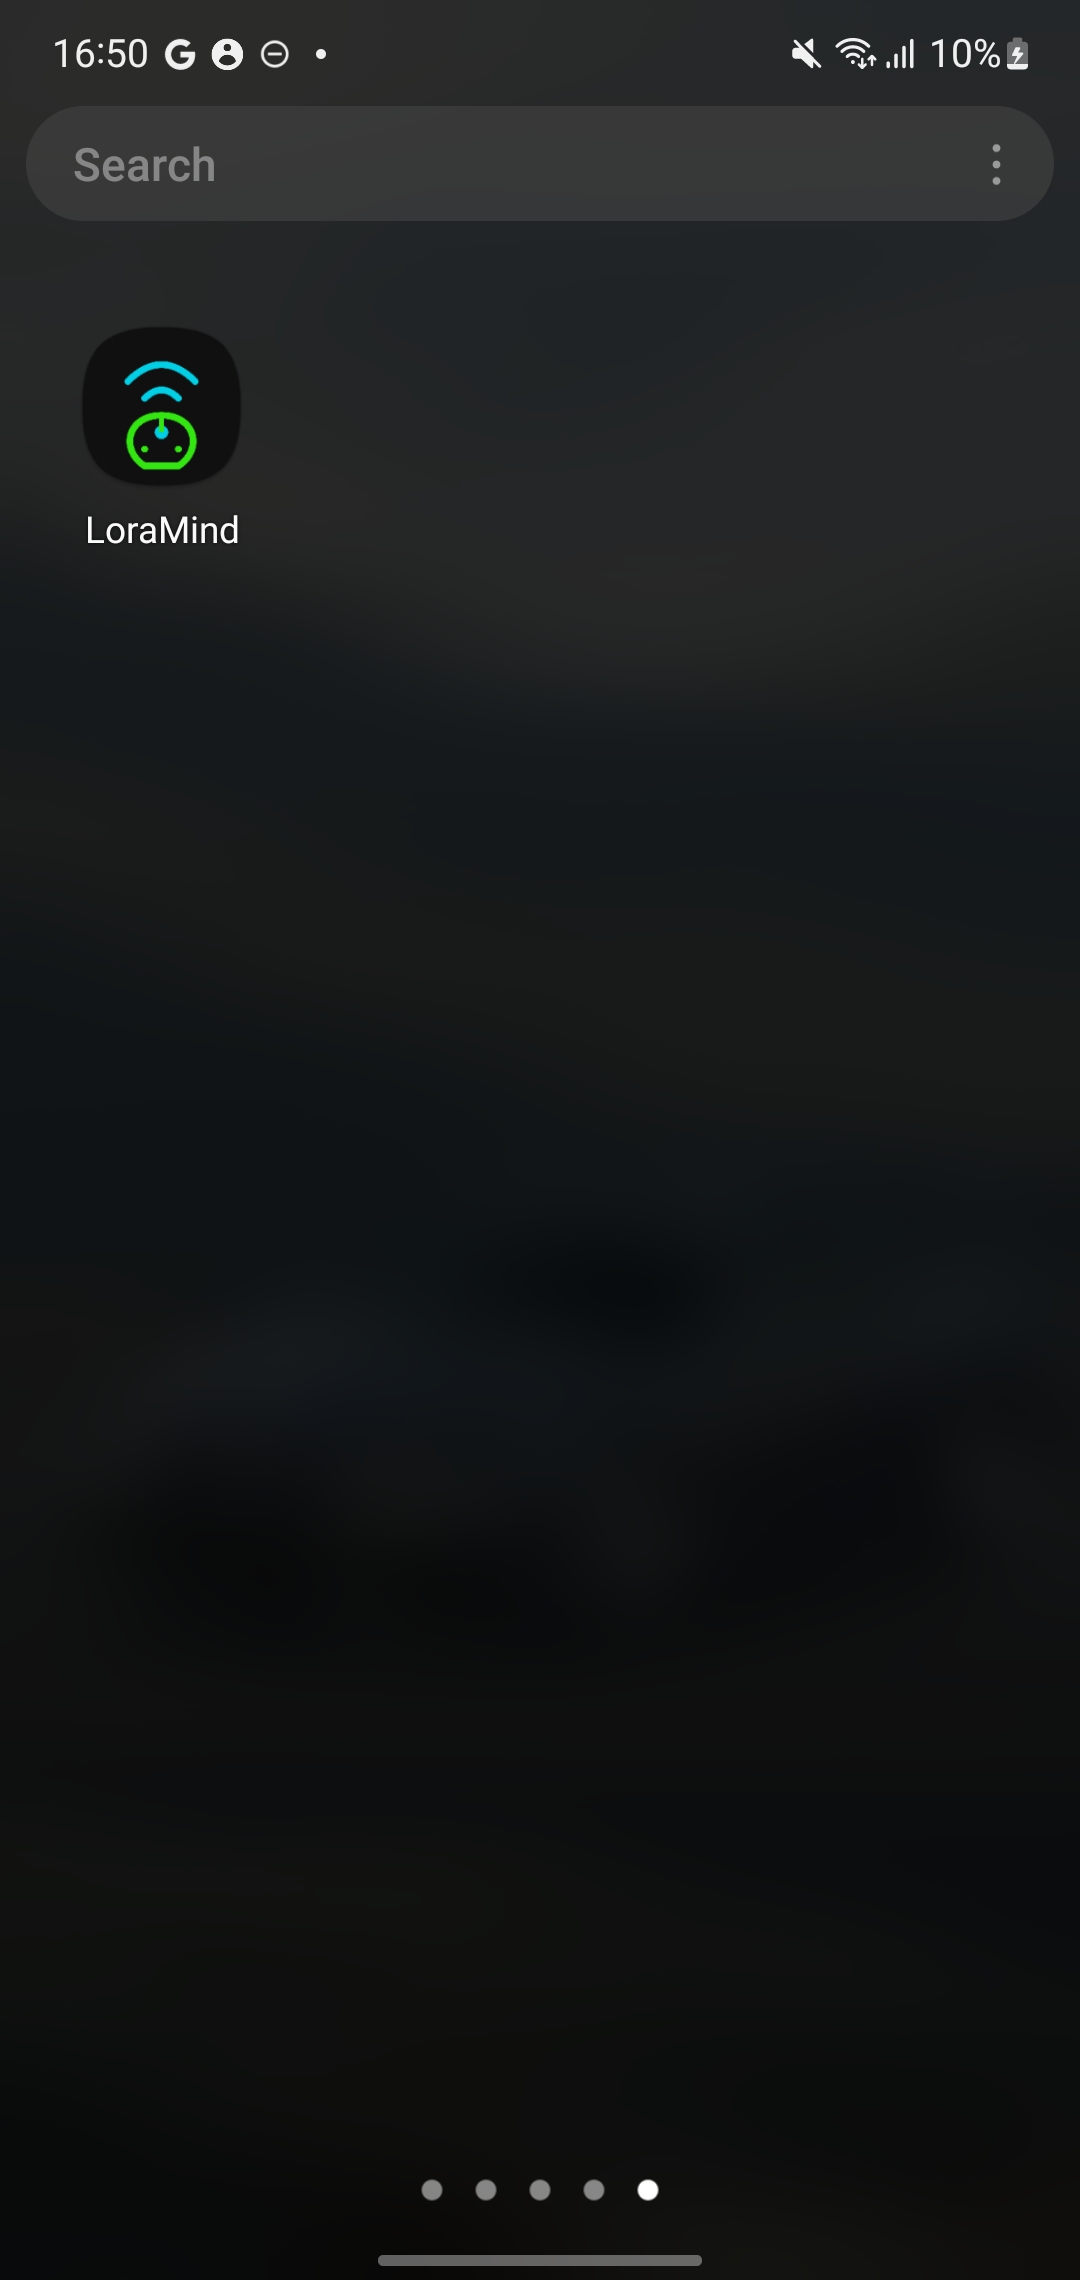
\includegraphics[width=0.68\linewidth]{figuras/interfaces/icone-app-grid.jpg}
        \par\smallskip\textbf{(a)} Ícone no menu de aplicativos.
    \end{minipage}
    \hfill
    \begin{minipage}[t]{0.46\textwidth}
        \centering
        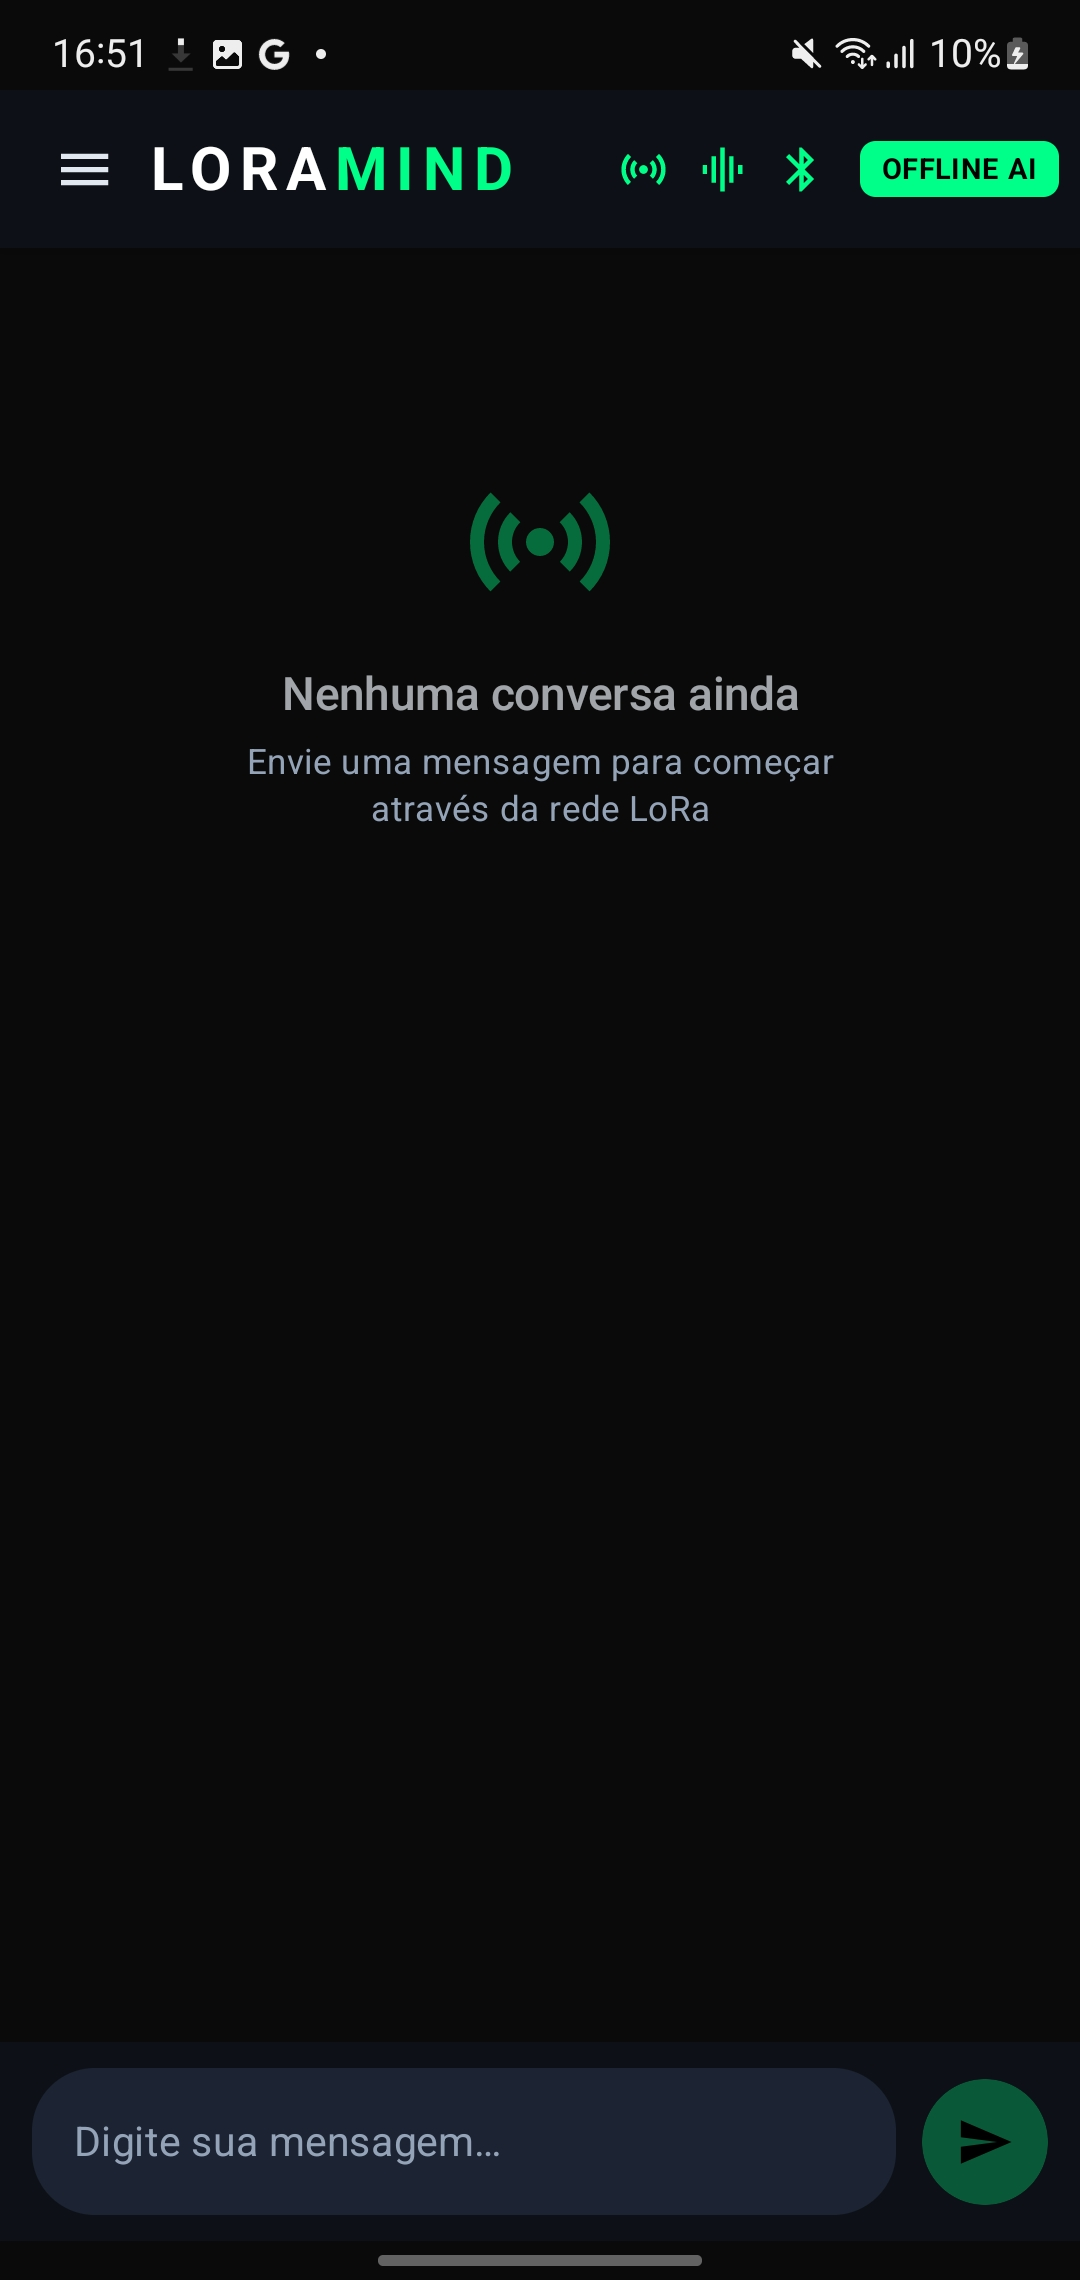
\includegraphics[width=0.68\linewidth]{figuras/interfaces/conversa-vazia.jpg}
        \par\smallskip\textbf{(b)} Estado inicial da conversa.
    \end{minipage}
    \caption{Acesso ao LoraMind e estado inicial da interface.}
    \label{fig:acesso-estado-inicial}
\end{figure}

\subsubsection{Tela Principal de Chat}

A tela principal concentra a interação do usuário com o sistema. As perguntas enviadas são alinhadas à direita e destacadas em verde, enquanto as respostas da inteligência artificial aparecem à esquerda em balões escuros. A indicação de entrega informa que a pergunta foi registrada pelo aplicativo. Quando uma resposta é dividida para transmissão, suas partes são apresentadas sequencialmente na mesma conversa, como pode ser observado na Figura~\ref{fig:conversa-historico}(a).

Enquanto a resposta é processada, a interface apresenta um indicador de espera e impede um novo envio. Quando o texto retorna pela conexão Bluetooth, ele é armazenado na conversa ativa e acrescentado à lista de mensagens, permitindo que o usuário acompanhe o diálogo em uma única tela.

\subsubsection{Barra Lateral e Histórico de Conversas}

A barra lateral é aberta pelo botão localizado no topo da tela ou por um gesto horizontal. Ela apresenta o botão para iniciar uma nova conversa e a lista das conversas armazenadas no aparelho. Cada item exibe o título e a data da última atualização, enquanto a conversa selecionada recebe um destaque visual. Ao tocar em um item, o aplicativo fecha a barra lateral e carrega somente as mensagens relacionadas à conversa escolhida. A Figura~\ref{fig:conversa-historico}(b) apresenta o histórico ao fundo do diálogo de exclusão.

\subsubsection{Exclusão de Conversas}

Para excluir uma conversa, o usuário mantém pressionado o respectivo item no histórico. Essa ação abre uma caixa de diálogo informando que todas as mensagens associadas também serão removidas, conforme a Figura~\ref{fig:conversa-historico}(b). O usuário pode cancelar a operação ou confirmá-la pelo botão de exclusão, reduzindo a possibilidade de apagamento acidental.

\begin{figure}[htbp]
    \centering
    \begin{minipage}[t]{0.46\textwidth}
        \centering
        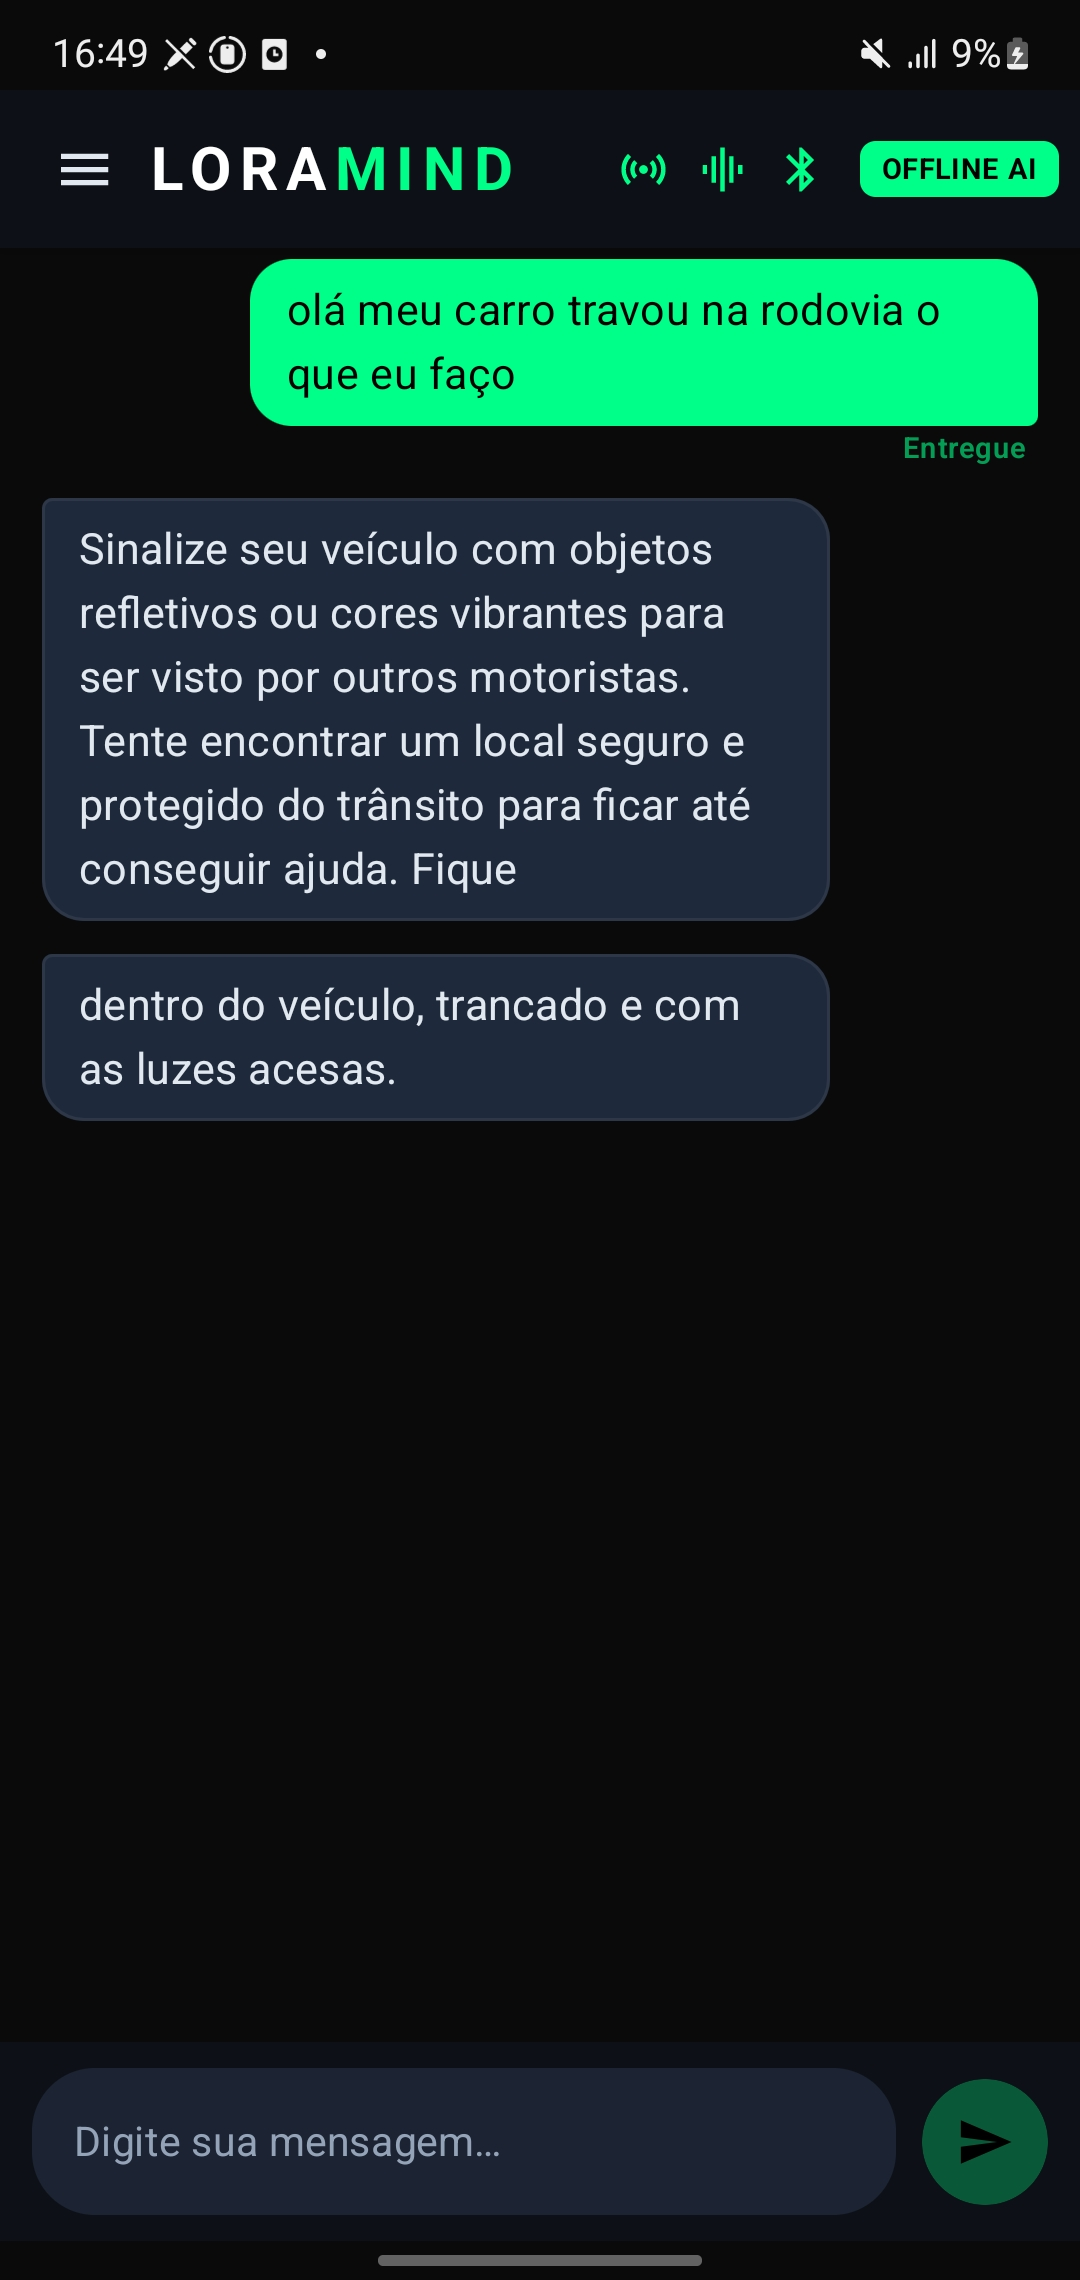
\includegraphics[width=0.68\linewidth]{figuras/interfaces/conversa-preenchida.jpg}
        \par\smallskip\textbf{(a)} Pergunta e resposta no chat.
    \end{minipage}
    \hfill
    \begin{minipage}[t]{0.46\textwidth}
        \centering
        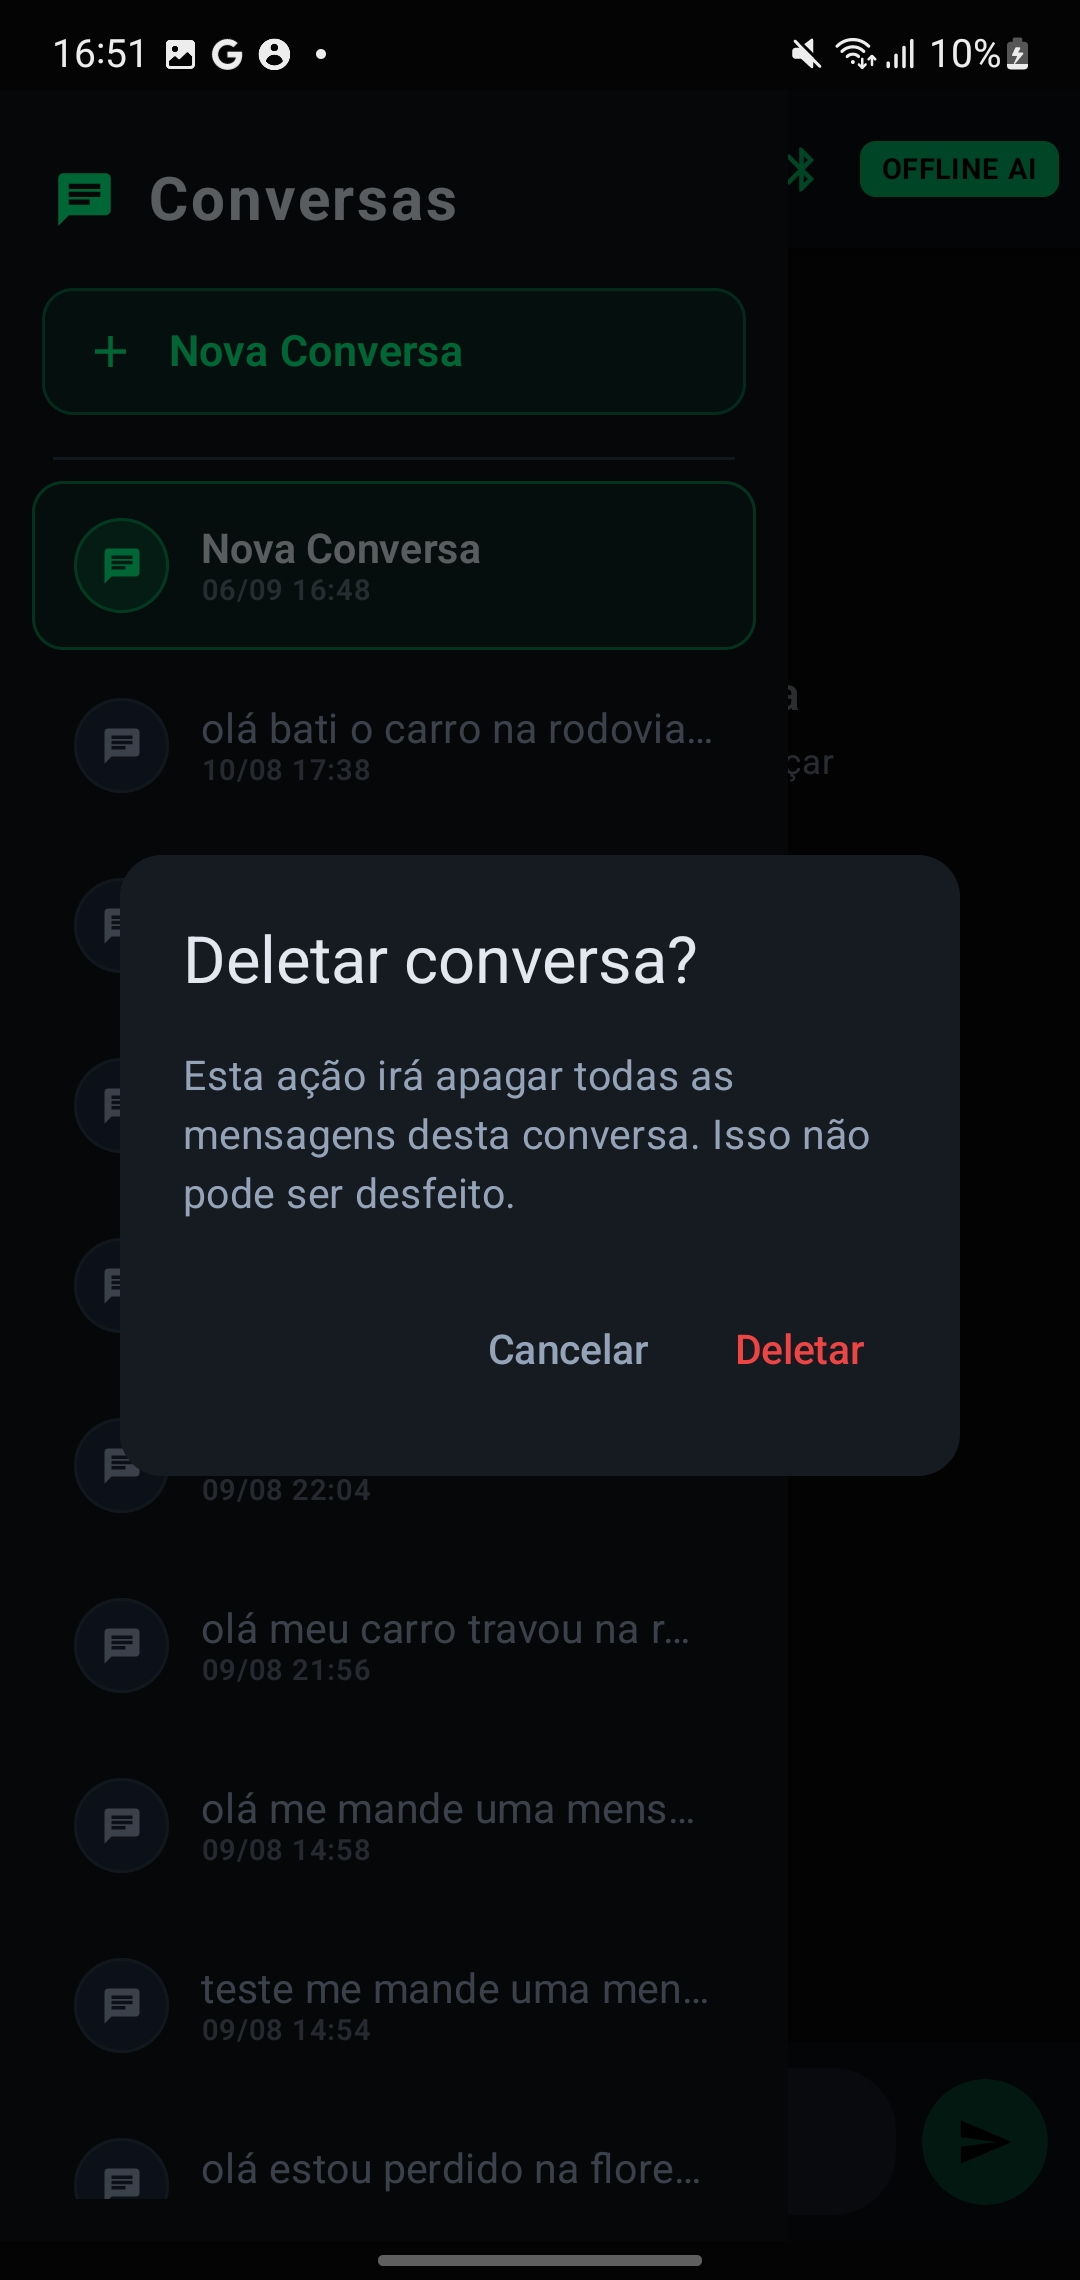
\includegraphics[width=0.68\linewidth]{figuras/interfaces/dialogo-exclusao.jpg}
        \par\smallskip\textbf{(b)} Histórico e confirmação de exclusão.
    \end{minipage}
    \caption{Conversa em andamento e gerenciamento do histórico.}
    \label{fig:conversa-historico}
\end{figure}

\subsection{Interface do Terminal no Computador}

No computador, a interação ocorre por meio do terminal em que o script \texttt{loramind\_bridge.py} é executado. Ao iniciar, ele apresenta a porta serial utilizada, o modelo carregado e o formato de comunicação esperado. Durante o funcionamento, cada linha recebe um horário e uma identificação visual, permitindo diferenciar mensagens informativas, avisos, erros, perguntas recebidas pela rede LoRa e respostas geradas pela inteligência artificial.

Quando uma pergunta válida chega pela estação-base, o terminal mostra o identificador da conversa, o \texttt{MSG\_ID} e o texto encaminhado ao modelo. A resposta é exibida progressivamente enquanto é produzida pelo Ollama. Após a conclusão, o terminal informa o tamanho do texto, a atualização do histórico e cada parte enviada ao ESP32. Essa interface auxilia no acompanhamento do fluxo e na identificação de problemas, mas não exige intervenção durante o uso normal do sistema.

% A imagem da interface do terminal será adicionada posteriormente.

\section{Avaliação do Projeto}
\label{sec:avaliacao-projeto}

\subsection{Metodologia de Avaliação}

A avaliação do LoraMind foi estruturada como uma validação técnica e funcional do protótipo completo. O objetivo foi verificar se os componentes apresentados na arquitetura conseguem operar de forma integrada e cumprir o fluxo proposto: receber uma pergunta no aplicativo, transportá-la até o computador, gerar uma orientação localmente e devolver a resposta ao usuário sem utilizar Wi-Fi ou dados móveis. A metodologia foi dividida em três eixos: comunicação e funcionamento ponta a ponta, comportamento do modelo local de inteligência artificial e funções da interface Android.

O ambiente de avaliação é composto por três dispositivos ESP32: dois atuam como nós da rede mesh destinados à conexão com dispositivos Android, e o terceiro corresponde à estação-base Heltec ESP32-S3 conectada ao computador por USB. O computador executa o script Python, o Ollama e o modelo Gemma 2 9B localmente. Para validar o encaminhamento da rede mesh, um segundo smartphone pode ser conectado ao outro nó ESP32, permitindo enviar mensagens a partir de pontos distintos. A mesma verificação também pode ser realizada pelos registros dos firmwares, que mostram o identificador, o tipo, o TTL e a decisão de entregar, retransmitir ou descartar cada pacote. Em conjunto com os registros do script Python, essas informações permitem acompanhar o percurso da mensagem e confirmar se a rede está tratando os pacotes corretamente.

\subsubsection{Comunicação e Fluxo Ponta a Ponta}

Os testes funcionais começam com o envio de perguntas pelo aplicativo em um smartphone sem acesso a Wi-Fi ou dados móveis. Para cada envio, verifica-se se o nó recebe o texto por Bluetooth, monta um pacote com identificador válido, transmite-o por LoRa e se a estação-base encaminha a pergunta ao programa Python. No retorno, observa-se se a resposta mantém o mesmo \texttt{MSG\_ID}, é transmitida pela rede LoRa e aparece na conversa correta do aplicativo.

Também são considerados casos em que a resposta precisa ser dividida em mais de um pacote. Nesse cenário, verifica-se se todas as partes são entregues, se pacotes repetidos são ignorados e se mensagens pertencentes a outro identificador não são apresentadas ao usuário incorreto. O tempo total é contado entre o envio no aplicativo e a exibição completa da resposta. A taxa de sucesso pode ser obtida pela razão entre o número de respostas completas recebidas e o total de perguntas enviadas.

Para observar o comportamento do enlace LoRa, os envios podem ser repetidos em diferentes distâncias e condições de visada. Em cada posição devem ser registrados a quantidade de tentativas, o recebimento completo da resposta, o RSSI e o SNR informados pelo firmware. Essa etapa permite avaliar o alcance do protótipo sem atribuir ao sistema a distância máxima teórica da tecnologia LoRa.

\subsubsection{Modelo Local de Inteligência Artificial}

A avaliação do modelo utiliza um conjunto fixo de perguntas dividido entre conhecimento geral e situações de risco, como pessoa perdida, ferimento ou veículo imobilizado. As respostas são verificadas segundo quatro critérios: relação com a pergunta, clareza, concisão e adequação ao cenário sem Internet ou telefonia. Nos casos de risco, também se observa se o modelo evita recomendar recursos indisponíveis e fornece ações que possam ser realizadas no local.

As mesmas perguntas podem ser submetidas ao \texttt{qwen2.5:3b} e ao \texttt{gemma2:9b}, mantendo o \textit{prompt} do sistema, para comparar qualitativamente o cumprimento das instruções. Além do conteúdo, os horários registrados pelo script permitem medir o tempo de geração. Essa comparação tem caráter funcional e não representa um \textit{benchmark} geral dos modelos, pois considera apenas os cenários e as configurações do LoraMind.

\subsubsection{Interface do Aplicativo Android}

A interface é avaliada por meio da execução das principais tarefas disponíveis ao usuário: abrir o aplicativo, iniciar uma conversa, enviar uma pergunta, aguardar a resposta, criar uma nova conversa, alternar entre históricos e excluir uma conversa. Para cada tarefa, verifica-se sua conclusão sem falhas, a atualização correta dos estados de espera e entrega e a associação das mensagens à conversa selecionada.

Também é verificado se as conversas permanecem disponíveis após fechar e abrir novamente o aplicativo e se a exclusão remove somente o histórico escolhido. Nesta etapa, a avaliação limita-se aos aspectos funcionais da interface no dispositivo utilizado para o protótipo; não foi conduzido um estudo formal de usabilidade com participantes.

\subsection{Resultados Obtidos}

Nos testes de alcance realizados com o protótipo, a comunicação LoRa permitiu a troca de perguntas e respostas a uma distância de aproximadamente 2~km. Nesse percurso, o sistema conseguiu transportar a mensagem do nó até a estação-base e devolver ao aplicativo a resposta produzida pelo modelo local, demonstrando a viabilidade da comunicação proposta para locais sem Wi-Fi ou cobertura de dados móveis.

A Semtech informa que enlaces LoRa podem alcançar até cerca de 5~km em áreas urbanas e 15~km ou mais em áreas rurais com linha de visada \cite{semtechrange2018}. Esses valores representam condições de referência e não uma distância garantida para qualquer implementação. No LoraMind, o alcance de aproximadamente 2~km ficou abaixo do limite urbano informado pelo fabricante. Essa diferença pode estar relacionada à interferência presente no ambiente, aos obstáculos entre os dispositivos, à posição e ao ganho das antenas e aos parâmetros adotados no protótipo. Ainda assim, o resultado obtido foi suficiente para comprovar o funcionamento do enlace no cenário avaliado.

\section{Considerações Finais}
\label{sec:consideracoes-finais}

\subsection{Resumo do Trabalho}

Este trabalho apresentou o LoraMind, um sistema que permite solicitar orientações a um modelo de inteligência artificial em situações nas quais o usuário não dispõe de acesso à Internet ou à rede de telefonia móvel. A solução transfere o processamento da inteligência artificial para um computador com maior capacidade e utiliza Bluetooth e LoRa para estabelecer a comunicação entre o aplicativo Android, os nós da rede e a estação-base.

O protótipo desenvolvido integrou o aplicativo Android, três dispositivos ESP32, uma rede mesh própria, o script de comunicação em Python e o modelo Gemma 2 9B executado localmente pelo Ollama. A troca completa de mensagens e o alcance de aproximadamente 2~km observado nos testes demonstram que a arquitetura é capaz de transportar perguntas e respostas sem depender de serviços de inteligência artificial na nuvem. A utilização de identificadores, TTL e deduplicação também permite que os nós encaminhem os pacotes e reconheçam quais respostas devem ser entregues a cada dispositivo.

Com isso, o projeto demonstra a possibilidade de combinar desenvolvimento móvel, sistemas embarcados, comunicação de longo alcance e inteligência artificial local em uma solução integrada. O LoraMind não elimina a necessidade de infraestrutura computacional, mas desloca essa infraestrutura para uma estação-base capaz de atender usuários próximos por meio da rede LoRa, reduzindo a dependência de conectividade convencional no ponto em que a orientação é solicitada.

\subsection{Contribuições do Trabalho}

\subsubsection{Contribuições Técnicas}

As contribuições técnicas deste trabalho estão relacionadas principalmente à integração dos componentes e à implementação do fluxo completo de comunicação. O projeto não propõe uma nova tecnologia de rádio ou um novo modelo de inteligência artificial, mas demonstra como recursos existentes podem ser combinados em uma solução voltada a ambientes com conectividade limitada. Entre as principais contribuições, destacam-se:

\begin{itemize}
    \item \textbf{Arquitetura integrada para comunicação com IA local:} desenvolvimento de um fluxo que conecta o aplicativo Android a um modelo executado em um computador, utilizando Bluetooth, dispositivos ESP32, comunicação LoRa e USB serial, sem depender de uma API de inteligência artificial na Internet;

    \item \textbf{Protocolo de aplicação sobre LoRa:} definição de uma estrutura de pacote com prefixo, tipo, identificador da mensagem, TTL e \textit{payload}, permitindo diferenciar perguntas e respostas, controlar retransmissões e reconhecer o dispositivo que aguarda cada resposta;

    \item \textbf{Encaminhamento em rede mesh:} implementação de retransmissão entre os nós, controle de TTL e deduplicação de pacotes, possibilitando ampliar a cobertura e evitar ciclos ou processamento repetido de mensagens;

    \item \textbf{Ponte entre a estação-base e o modelo:} criação de um script Python que identifica a porta serial, interpreta as mensagens recebidas, mantém o histórico separado por conversa, consulta a API local do Ollama e divide respostas extensas em partes adequadas à transmissão;

    \item \textbf{Aplicativo Android com persistência local:} implementação de uma interface de chat organizada com Clean Architecture e MVVM, capaz de armazenar conversas e mensagens, acompanhar respostas recebidas por Bluetooth e preservar o histórico mesmo sem conexão com a Internet.
\end{itemize}

\subsubsection{Contribuições Sociais}

As contribuições sociais do LoraMind são apresentadas como possibilidades decorrentes da solução desenvolvida, pois o protótipo ainda não foi avaliado em situações reais de emergência ou por um grupo de usuários. Nesse contexto, destacam-se:

\begin{itemize}
    \item \textbf{Acesso a orientações em áreas sem conectividade convencional:} possibilidade de enviar perguntas e receber um direcionamento inicial em locais nos quais não há cobertura de Internet ou telefonia móvel;

    \item \textbf{Redução da dependência do poder computacional do smartphone:} execução do modelo de inteligência artificial em uma estação-base, permitindo que o aplicativo seja utilizado em dispositivos Android que não possuem capacidade suficiente para executar localmente um modelo desse porte;

    \item \textbf{Compartilhamento da infraestrutura:} possibilidade de uma estação-base atender diferentes usuários conectados aos nós da rede LoRa, concentrando o custo computacional em um único ponto;

    \item \textbf{Aplicação em cenários de isolamento:} potencial de utilização em áreas rurais, trilhas, regiões remotas ou locais afetados por falhas temporárias na infraestrutura de comunicação.
\end{itemize}

O sistema fornece somente um direcionamento inicial com base na resposta de um modelo de linguagem. Portanto, não substitui profissionais, autoridades ou serviços de emergência quando esses recursos estiverem disponíveis.

\subsection{Limitações Identificadas}

Apesar do funcionamento obtido pelo protótipo, foram identificadas limitações relacionadas à rede mesh, à execução local da inteligência artificial e ao enlace LoRa:

\begin{itemize}
    \item \textbf{Limite de saltos da rede mesh:} os pacotes são criados atualmente com TTL igual a três, permitindo no máximo três retransmissões antes do descarte. Esse limite foi adotado para impedir que uma mensagem permaneça circulando na rede e para reduzir a ocorrência de loops. Entretanto, ele também restringe o tamanho da rota, pois um dispositivo que dependa de mais de três nós intermediários pode não receber a pergunta ou a resposta;

    \item \textbf{Dependência do hardware para execução da IA:} como o modelo é executado localmente, sua capacidade fica condicionada à memória e ao poder de processamento do computador conectado à estação-base. O Gemma 2 9B foi escolhido por ser compatível com o equipamento disponível, porém modelos maiores e potencialmente mais capazes exigiriam mais memória, capacidade gráfica e tempo de processamento;

    \item \textbf{Interferência na comunicação LoRa:} o alcance e a estabilidade da comunicação podem ser reduzidos por interferências, obstáculos, relevo, posicionamento das antenas e outros sinais na mesma faixa de frequência. Em ambientes desfavoráveis, essas condições podem causar perda de pacotes, necessidade de retransmissões ou impedir a comunicação mesmo em distâncias inferiores aos valores de referência da tecnologia.
\end{itemize}

\subsection{Trabalhos Futuros}

Com base nas limitações observadas, algumas melhorias podem ampliar a confiabilidade e a capacidade do LoraMind:

\begin{itemize}
    \item \textbf{Controle de repetição por nó:} substituir o limite fixo de três saltos por um mecanismo no qual cada ESP32 registre os identificadores dos pacotes já processados. Assim, um nó descartaria uma mensagem ao recebê-la novamente, evitando loops sem limitar previamente a quantidade total de saltos. Essa abordagem permitiria redes maiores, embora exigisse mais memória e processamento dos dispositivos para manter e consultar esse histórico;

    \item \textbf{Utilização de um modelo de IA mais robusto:} empregar um computador com maior capacidade de processamento e memória para executar modelos mais avançados. Além de melhorar a qualidade das respostas, essa evolução permitiria explorar técnicas mais elaboradas de engenharia de prompt e fornecer instruções mais específicas para os cenários atendidos pelo sistema;

    \item \textbf{Confirmação de entrega e retransmissão:} adicionar mensagens de confirmação entre os nós para identificar pacotes que não chegaram ao destino e realizar novas tentativas de envio. Esse mecanismo pode tornar a comunicação mais confiável em ambientes com interferência, desde que seja controlado para não aumentar excessivamente o tráfego da rede;

    \item \textbf{Segurança das mensagens:} implementar autenticação e criptografia dos pacotes para impedir a leitura ou a alteração das perguntas e respostas por dispositivos não autorizados. Essa melhoria é especialmente relevante caso o sistema seja utilizado para transmitir informações pessoais ou relacionadas a situações de risco;

    \item \textbf{Avaliação em cenários mais amplos:} realizar testes com mais nós, diferentes distâncias, obstáculos e níveis de interferência. Esses experimentos permitiriam medir com maior precisão o alcance, o tempo de resposta, a perda de pacotes e a escalabilidade da rede mesh.
\end{itemize}

\subsection{Conclusão}

Os resultados obtidos indicam que o objetivo de desenvolver um sistema capaz de conectar usuários a um modelo local de inteligência artificial sem depender de Wi-Fi ou dados móveis foi alcançado. O protótipo realizou o fluxo completo entre o aplicativo Android e a estação-base, transportando perguntas e respostas por Bluetooth, por uma rede mesh LoRa e pela comunicação serial com o computador. Nos testes realizados, o enlace LoRa permaneceu funcional a aproximadamente 2~km, demonstrando a viabilidade técnica da proposta no cenário avaliado.

O LoraMind deve ser compreendido como um protótipo experimental. O alcance da comunicação está sujeito às condições do ambiente, a rede ainda utiliza um limite fixo de saltos e a qualidade das respostas depende do modelo e do hardware disponíveis na estação-base. Além disso, as orientações produzidas pela inteligência artificial não substituem profissionais, autoridades ou serviços de emergência.

Ainda assim, o trabalho demonstra que a integração entre dispositivos móveis, sistemas embarcados, comunicação LoRa e inteligência artificial local pode oferecer uma alternativa de acesso a informações em regiões com conectividade limitada. As melhorias propostas poderão aumentar a cobertura, a confiabilidade e a segurança da solução, permitindo sua avaliação futura com mais dispositivos e em situações de uso mais próximas das condições reais.

\section{Agradecimentos}

Agradeço ao meu orientador, Prof. Ademar T. Akabane, pelo acompanhamento, pelas orientações e pelas contribuições realizadas durante o desenvolvimento deste trabalho. Agradeço também aos professores da Pontifícia Universidade Católica de Campinas pelos conhecimentos compartilhados ao longo da graduação e pelo apoio à minha formação acadêmica e profissional.

Por fim, agradeço à minha família, aos meus amigos e a todos que me apoiaram durante essa trajetória, oferecendo incentivo, compreensão e colaboração para que este trabalho pudesse ser concluído.

% Mantém as referências numeradas conforme a ordem da primeira citação.
\bibliographystyle{unsrt}
\bibliography{sbc-template}

\end{document}
  
